\documentclass[12pt, letter]{article}
\usepackage{graphicx} % Required for inserting images
\usepackage{dirtree}
%\usepackage{biblatex}

%\addbibresource{report.bib}

\graphicspath{{Report_Images/}}
\title{Project Report:
Mini Game Hub}
\author{Chinmaya Shankara Shastry  and Arnav Singh }
\date{April 29, 2026}

\begin{document}

\maketitle
\newpage
\tableofcontents
\newpage

\section{Introduction}
Our project is a secure, multi-user game hub that utilizes Bash scripting for authentication and Python for gameplay using the Pygame library. In it, two authenticated players select a game from a menu, play via a graphical interface, and have their results recorded on a persistent leaderboard.

\section{External Libraries}

\subsection{Pygame-ce}
Pygame is the core of the whole project. It provides a GUI for the user to interact with the project and play the game, and is also used to handle the implementation of all the features. \cite{pygame}


\subsection{Numpy}
In this project, we used the numpy library to handle the core logic behind each of the board games we implemented. We stored the gameboard state as a numpy array, upon which operations were performed corresponding to moves in the game. Finally, we checked the win condition by applying various numpy functions and operations to the array. \cite{numpy}

\subsection{Matplotlib}
We have used the Matplotlib library to display graphs based on the game statistics saved in history.csv. When called, 2 bar graphs and a pie chart are displayed with relevant statistics. \cite{matplotlib}

\section{Design and Architecture}

\subsection{System Overview}
The project is designed as a modular system with multiple components which separates authentication, gameplay and analytics into separate layers. The system begins with a Bash script (main.sh) which authenticates both users, after which control is passed to the Python-based game engine(game.py) which handles game selection, gameplay and processing of the game results. After a game is played, its results are recorded, which are used to generate statistics which are displayed using leaderboard.sh and matplotlib(via game.py).

\subsection{Game Engine Design}
\subsubsection{Base Class Abstraction}
The core of the system is a generic base class, contained in the file game\_class.py This generic class represents a two-player, turn based board game. This class covers all the common functions, properties and methods used across the games in the project. 

The common properties include \texttt{gameboard, p1, p2, turn, winner} which are the array representing the game board, player 1, player 2, the current turn and the winner of the game respectively. The common methods include:
\begin{itemize}
    \item \texttt{switch\_turn()}: This function switches the turn variable from one player to another.
    \item \texttt{make\_move(move)}: This function puts a piece of the current player on the board at the indices given in move, this is redefined in some child classes.
    \item \texttt{check\_win\_condition()}: This function is just an abstract, it is defined in all subclasses as it is different for each game.
    \item \texttt{render\_av(pos,player)}: This function is used to render the specified player's avatar at the position pos.
\end{itemize}
\subsubsection{Inheritance Structure}
Each game is implemented as a subclass of the base class Game. The subclasses implemented in our project are TicTacToe, Othello, Connect4, Chain\_rxn and Checkers, however any number of games can conveniently be implemented as subclasses of the base class Game.

Each subclass defines how to render its own board and pieces in the main game loop with \texttt{renderboard()}, overrides the \texttt{check\_win\_condition()} method in the base game class with its own logic, and implements the functions needed for making moves according to the game's logic.
%maybe make this a list?

\subsubsection{TicTacToe Class}
%insert logic here
In the TicTacToe class, the game board is stored as a Numpy array, the same as all the other games. In TicTacToe, the pieces of player 1 are represented with 1, the pieces of player 2 are represented with 2 and all the empty squares are represented by 0.

The functions defined in the TicTacToe class apart from the ones in its parent class Game are as follows:
\begin{itemize}
    \item \texttt{renderboard()}: This function renders the board and pieces of the game, as well as the surrounding elements(including boxes, avatars and player name text) according to the board size given during initialization of the class. It renders the pieces different colours based on the player.
    \item \texttt{checkpress(click)}: This function, given click event, checks where on the gameboard it was clicked and executes the appropriate action. If that position on the board has a piece already it does nothing otherwise  it will call the \texttt{make\_move} function which will make the move to that position. Then \texttt{check\_win\_condition} is called to check if the current player won if not then the turn is switched.
    \item \texttt{check\_win\_condition(move)}: This function takes the location of the played move as input and uses numpy slicing to obtain the row, column and both diagonals through that square. It then compares each of those slices with 4 offset slices and checks if any element in the output is equal in all the slices using .any(). If this is the case it means that element is the beginning of a 5 in a row hence determining the winner. In case the board is full this function returns -1 to represent a draw.
\end{itemize}
\subsubsection{Othello Class}
%insert logic here
In the Othello class, the game board is stored as a Numpy array, the same as all the other games. In Othello, the pieces of player 1 are represented with 1, the pieces of player 2 are represented with 2 and all the empty squares are represented by 0.

The functions defined in the Othello class apart from the ones in its parent class Game are as follows:
\begin{itemize}
    \item \texttt{renderboard()}: This function renders the board and pieces of the game, as well as the surrounding elements(including boxes, avatars and player name text) according to the board size given during initialization of the class. It renders the pieces different colours based on the player.
    \item \texttt{check\_list(arr, pos, player)}: This function checks if the move played at position pos by the current player in array arr follows othello rules or not. It does so by using the numpy.argwhere function to find the closest position which is the same as the player and uses slicing and .any() to check if the there are any empty squares between this closest position and the played position. If there are empty squares the move is invalid and the function returns false otherwise it returns true.
    \item \texttt{valid\_move(self,move0,move1,player)}: This function takes the move and the player who played it as arguments and uses slicing to find every diagonal, column and row through the position of played move. It then passes the sliced array, position of played move in the sliced array and player to \texttt{check\_list} to see if any of them contains a valid set of flips.
    \item \texttt{has\_moves()}: This is the output when numpy.vectorize is applied to \texttt{valid\_move} and it takes the array containing x coordinates of every empty square, array containing y coordinates of every empty square and current player as arguments. These arrays are found using numpy.argwhere() and the output of texttt{has\_moves} is an array containing True if the square at that x, y has a valid move and False otherwise.
    \item \texttt{possible\_moves()}: This function uses \texttt{has\_moves} to give a list of indices where the gameboard has valid moves and is used in \texttt{renderboard()} to visually represent them.
    \item \texttt{make\_move(move)}: This function is called only if the played move is valid. It checks every row, column, diagonal through the position of played move and checks if it contains valid flips. If it the sliced array contains valid flips it updates the gameboard by flipping all of the opponents pieces at the specified locations and finally places the current player's piece at the input location.
    \item \texttt{checkpress(click)}: This function, given click event, checks where on the gameboard it was clicked and executes the appropriate action. If that position on the board has a piece already or is an invalid move by othello rules it does nothing otherwise  it will call the \texttt{make\_move} function which will make the move to that position and flip all the opponents pieces which are to be flipped. Then \texttt{check\_win\_condition} is called to check if the current player won if not then the turn is switched. If the opponent has no valid moves the turn is switched back.
    \item \texttt{check\_win\_condition()}: This function checks if there are any valid moves left for either player or if the board is full, in case of no moves left it counts the number of pieces of each player using numpy.argwhere() and in the case both have equal number of pieces it returns -1 to represent draw.
\end{itemize}
\subsubsection{Connect4 Class}
%insert logic here
In the Connect4 class, the game board is stored as a Numpy array, the same as all the other games. In Connect4, the pieces of player 1 are represented with 1, the pieces of player 2 are represented with 2 and all the empty squares are represented by 0.

The functions defined in the Connect4 class apart from the ones in its parent class Game are as follows:
\begin{itemize}
    \item \texttt{renderboard()}: This function renders the board and pieces of the game, as well as the surrounding elements(including boxes, avatars and player name text) according to the board size given during initialization of the class. It renders the pieces different colours based on the player.
    \item \texttt{checkpress(click)}: This function, given click event, checks where on the gameboard it was clicked and executes the appropriate action. If the column to which the position belongs is full it does nothing otherwise  it will call the \texttt{make\_move} function which will make the move to the appropriate position. Then \texttt{check\_win\_condition} is called to check if the current player won if not then the turn is switched.
    \item  \texttt{make\_move(move)}: This function receives the location of the mouseclick and enters the current players representative number in the lowest unoccupied square belonging to the column where the move was played.
    \item \texttt{check\_win\_condition(move)}: This function takes the location of the played move as input and uses numpy slicing to obtain the row, column and both diagonals through that square. It then compares each of those slices with 3 offset slices and checks if any element in the output is equal in all the slices using .any(). If this is the case it means that element is the beginning of a 4 in a row hence determining the winner. In case the board is full this function returns -1 to represent a draw.
\end{itemize}

\subsubsection{Chain\_rxn Class}
%insert logic here
In the Chain\_rxn class, the game board is stored as a 3-Dimensional Numpy array. In Chain\_rxn, the pieces of player 1 are represented with [1, number of atoms], the pieces of player 2 are represented with [2, number of atoms] and all the empty squares are represented by [0,0].

The functions defined in the Chain\_rxn class apart from the ones in its parent class Game are as follows:
\begin{itemize}
    \item \texttt{renderboard()}: This function renders the board and pieces of the game, as well as the surrounding elements(including boxes, avatars and player name text) according to the board size given during initialization of the class. It renders the pieces different colours and numbers based on the player, atom count.
    \item \texttt{make\_move(move)}: This function is called if the location 'move' is empty or has atoms of the same colour as the player. If the position is empty \texttt{make\_move} places one atom of the players colour in that position. If the position is not empty \texttt{make\_move} adds an atom as long as it doesnt exceed the atom limit of that square. If the atom limit is exceeded \texttt{make\_move} is recursively called for adjacent squares. Since in some cases it is not possible for all squares to contain lesser atoms than their limit, \texttt{check\_win\_condition} is called after the recursive call as well to prevent reaching max recursion depth. 
    \item \texttt{checkpress(click)}: This function, given click event, checks where on the gameboard it was clicked and executes the appropriate action. If that position contains atoms belonging to other player nothing is done  otherwise  it will call the \texttt{make\_move} function which will make the move to that position, and any subsequent explosions as well. Then \texttt{check\_win\_condition} is called to check if the current player won if not then the turn is switched.
    \item \texttt{check\_win\_condition(move)}: This function 
    uses np.argwhere() to check if any squares are left containing the opponent's atoms. If no such squares are left it returns the current player's representative number. If squares are left it returns 0 to indicate the game is ongoing. In this game draws are not possible and one player is guaranteed to lose.
\end{itemize}
\subsubsection{Checkers Class}
%insert logic here
In the Checkers class, the game board is stored as a Numpy array, the same as all the other games. In Checkers, the pieces of player 1 are represented with 1 and -1, where 1 is a normal piece and -1 is a "king" piece which can also move backward. Similarly, the pieces of player 2 are represented with 2 and -2 and all the empty squares are represented by 0.
There is also a self.selected attribute which stores which piece has currently been selected as a pair of indices.

The functions defined in the Checkers class apart from the ones in its parent class Game are as follows:

\begin{itemize}
    \item \texttt{renderboard()}: This function renders the board and pieces of the game, as well as the surrounding elements(including boxes, avatars and player name text) according to the board size given during initialization of the class. It renders the pieces different colours based on the player and also adds a marker for the "king" pieces in checkers. It also ensures that the selected piece is rendered in a slightly darker shade, so that the player knows which piece is making the move.
    
    \item \texttt{check\_existence(i,j)}: This function, given the indices i,j of a piece in the game board will return whether there exists a valid move for that piece. It returns True if there is a valid move and returns False if there does not or if that position does not have a piece. Depending on whose turn it is and the type of piece(king or normal) it checks the existence of direct and jumping moves (i.e. if the immediately adjacent square is empty or if it is occupied, the square directly diagonal to that is empty), and returns a boolean value.
    
    \item \texttt{jump(pos)}: This function checks for the availability of jumps for the piece at the position pos. If a jump exists, it makes the piece perform that jump, and recursively calls jump again. If a jump does not exist, it returns False and stops the recursion(if any). It checks for jumps in all 4 directions, and executes a jump if it finds one. It also changes the piece into a king if it reaches the end of the board. 
    
    \item  \texttt{make\_move(move)}: This function checks if the given move is valid. If it is valid, it executes the move and any follow-ups if required. For example, if the move makes the piece land on the last row of the board, it turns that piece into a king, or if a jump is executed, it calls the \texttt{jump} function to execute serial jumps. It checks the direction of the move(with respect to original position) and if it is a valid direction(forward for normal pieces, forward and backward for king pieces) for normal moves and for jumps, and if the direction is valid and the move exists, it makes the move.
    \item \texttt{checkpress(click)}: This function, given click event, checks where on the gameboard it was clicked and executes the appropriate action. If that position on the board has a piece which was not previously selected(and also belongs to the current player), it will check if that piece has a valid move using the \texttt{check\_existence} function. If it has a valid move, then that piece will get selected. If a piece is already selected, it will call the \texttt{make\_move} function which will make the move to that position only if the move exists. If a move is made, the turn will be changed and the function \texttt{check\_win\_condition} will be called.
    \item \texttt{check\_win\_condition()}: This function checks the board for a winner using Numpy functions, if it finds a winner it will return an integer corresponding to the winner (1 for player 1 and 2 for player 2). The function checks if the opposing player is out of pieces or if they do not have valid moves using a vectorized version of the function \texttt{check\_existence}.
\end{itemize}

\subsection{Storage}
There are 2 primary files being used to store data:
\begin{itemize}
    \item \texttt{users.tsv}: Stores usernames, SHA-256 hashed passwords and data related to avatars
    \item \texttt{history.csv}: Stores game results in the format: Win/Draw, Game name, Winner, Loser, Date
\end{itemize}

\subsection{Control Flow}
The game engine operates as a loop with multiple state variables, depending on which the relevant code is executed. It switches between different menu modes, the gameplay mode and the analytics state where the graphs are displayed using matplotlib. After each game, the game results are appended to history.csv and leaderboard.sh is called and graphs are displayed(if the user chooses to do so).
\section{Features Implemented}

\subsection{Authentication}
Authentication is done by using the Login() function and its helper functiions. The general template for each one of them is a while loop which runs as long as the input is incorrect or has invalid formats (such as incorrect, length, lack of strong password etc.). In case the players have used GameHub before their inputted passwords are compared with those stored in users.tsv (hashed) and allowed access accordingly.
main.sh then calls game.py along with the 2 players' names as arguments.

\subsection{Leaderboard}
leaderboard.sh is called by game.py when the user is prompted post game or if the user navigates to it through the analytics menu. When sorted by wins in case of a tie the person with more losses is ranked lower. When sorting by losses the person with more wins in a tie is ranked lower. When sorted by win loss ratio all people with 0 losses are ranked by wins higher than the rest. People with a w/l ratio of 0 are ranked higher than players with 0 wins and 0 losses who are also designated a w/l ratio of 0. The ties for draws are also decided by wins. The leaderboard displays the top 5 in each category for each game as displaying every single user would take up too much space on the terminal and it might not even be possible to scroll that much.

\subsection{Games}

\subsubsection{TicTacToe}
The rules of the game are as follows:
\begin{itemize}
    \item Both players make moves with X and O(blue and red circles in our project).
    \item The first player to get 5 in a row is considered the winner
    
\end{itemize}
In our project, we have implemented a version of Tic-Tac-Toe which is played on a 10x10 grid, and when a player gets 5 in a row we consider it as a win.

\subsubsection{Othello}
The rules of the game are as follows:
\begin{itemize}
    \item Each player plays moves in squares as long as the played move traps the opponent's pieces between it and a priorly placed piece. 
    \item All the trapped pieces are then flipped to the current player's colour.
    \item If a player has no valid moves his turn gets skipped.
    
\end{itemize}
This goes on till both players cannot make moves after which their pieces are counted and the one with more pieces wins.

\subsubsection{Connect4}
The rules of the game are as follows:
\begin{itemize}
    \item Players drop their pieces in their desired column.
    \item Pieces cannot be placed in squares if there is no piece below it.
    \item The first player to get 4 of his pieces in a row in any direction is the winner.
    
\end{itemize}


\subsubsection{Chain Reaction}
The rules of the game are as follows:
\begin{itemize}
    \item Each square has a limit on number of atoms. Corner - 1, Edge - 2, Central - 3.
    \item Players take turns playing atoms into squares which are empty or contain their atoms.
    \item If a square exceeds its limit it "explodes" which means it becomes empty and all neighbouring squares gain one atom.
    \item If the neighbouring squares now exceed their limits they too will explode.
    \item The game is played till one of the players is completely wiped off the board.
    
\end{itemize}
It is important to realize that draws are not possible in this game and a winner is guaranteed.


\subsubsection{Checkers}
The rules of the game are as follows:
\begin{itemize}
    \item Pieces can only move diagonally. Normally pieces can move only diagonally forward, but "Kings" can move both forward and backward.
    \item Pieces can either move 1 square diagonally, or can jump over a piece of the opposing player to move 2 squares diagonally. If this is done, the opposing piece is removed. After a jump, if any other jumps are possible the player must take them.
    \item Players take turns making moves like this. When a piece reaches the edge of the board it becomes a "king".
    
\end{itemize}
Play continues until one of the players is out of pieces or has no moves left, at which point he is said to have lost.

\subsection{Background}
The background consists of lines of "code" moving down at different speeds at different locations to replicate the code rain from the movie "The Matrix". This effect was created by getting 15 images of said lines of "code" and randomly designating one of the 15 to each interval created by splitting the width of the screen into intervals of width 20 px. The images are then given a random offset and a random speed parameter. The images are blitted 1 * (speed parameter) px lower in each iteration of the loop to give the effect that it is moving down.

\subsection{Menu bar/Selection menus}
We have implemented a menu bar and selection menus as part of the game UI. As you can see in Fig. 1, the main landing screen has a menu bar with three buttons. When you click either one of the "Options" or the "Play" buttons, it opens up a menu with various options which you can choose from. This is detailed later on.

\subsection{Avatar system}
We have implemented an avatar system in which each player can assign themselves an avatar through the game UI. After opening "Options", once you click on "Avatar"  it opens an interface through which the player can customize their avatar.

It includes options for customizing the colour of the avatar, the hat of the avatar, the eyes/eyewear of the avatar and the mouth of the avatar. This can be done for both players by switching between them. The various aspects of the avatar are stored as separate images and the choices of each player are stored in users.tsv as numbers from 0 to 4 for each individual characteristic. These separate images are then blitted sequentially to make the entire avatar.

The avatars are also displayed on either side of the board during a game and are highlighted when it is that player's turn to notify them to make a move. They are also briefly displayed on the win screen which pops up right after a game is finished.

\subsection{Background music playback system}
We have also implemented a background music playback system in which the players can switch betweeen different music tracks which loop in the background. The players can also change the volume of the background music.
\newpage
\section{Directory Structure}
\dirtree{%
.1 GameHub/. 
.2 Graphics/ \quad Contains all the image files used in the project.
.2 Sound/ \quad Contains all the music/sound files used in the project.
.2 Report\_Images \quad Contains all the image files used in the report.
.2 hub/.
.3 game.py \quad Main game engine and UI.
.3 leaderboard.sh \quad Processes history.csv and displays leaderboard.
.3 main.sh \quad Authentication and entry point .
.3 history.csv \quad Stores game results.
.3 users.tsv \quad Stores user credentials (hashed with SHA-256).
.3 games/.
.4 avatar\_render.py \quad Used for avatar rendering.
.4 chain\_rxn.py \quad Chain Reaction game class.
.4 checkers.py \quad Checkers game class.
.4 connect4.py \quad Connect Four game class.
.4 game\_class.py \quad Base game class.
.4 othello.py \quad Othello game class.
.4 text.py \quad Text rendering utilities.
.4 tictactoe.py \quad Tic-Tac-Toe class.
.3 utilities/.
.4 analytics.py \quad Handles statistics and plots.
.4 avatar\_menu.py \quad Avatar selection menu.
.4 button.py \quad Button class used in UI.
.4 sound.py \quad Sound selection menu.
.2 Makefile \quad Makefile for report.
.2 report.bib \quad Bibliography file for report.
.2 report.pdf \quad Report PDF file.
.2 report.tex \quad Report Latex file.
.2 README.md \quad Project documentation.
.2 SpaceMono-Regular.ttf \quad Font used in project.
}
\newpage

\section{Installation and Setup}
\subsection{System Requirements}
\begin{itemize}
    \item Python 3.10
    \item Bash shell(Linux works best, running with WSL creates minor issues)
\end{itemize}
\subsection{Python Dependencies}
The following commands must be run in bash shell
\begin{verbatim}
    pip install pygame-ce
    pip install numpy
    pip install matplotlib
\end{verbatim}
All the required sound files and images needed for the game are already included, no additional setup is required. To run the project, use \texttt{bash main.sh}.


\section{Usage}
\textbf{This project should only be run on Linux for complete functionality.
If not, there may be issues with the sound, the avatar system and/or the matplotlib functionality. Do not resize the window, this will cause issues with the background and will also skew the positioning of the elements.}

The project can be run by \texttt{bash main.sh} in the directory hub upon which both players will be prompted to sign in using their usernames and passwords, and to create a new username if this is their first time.

After this, the python script game.py will be called, opening a landing screen which is displayed in the screenshot below.
\begin{figure}[h]
    \centering
    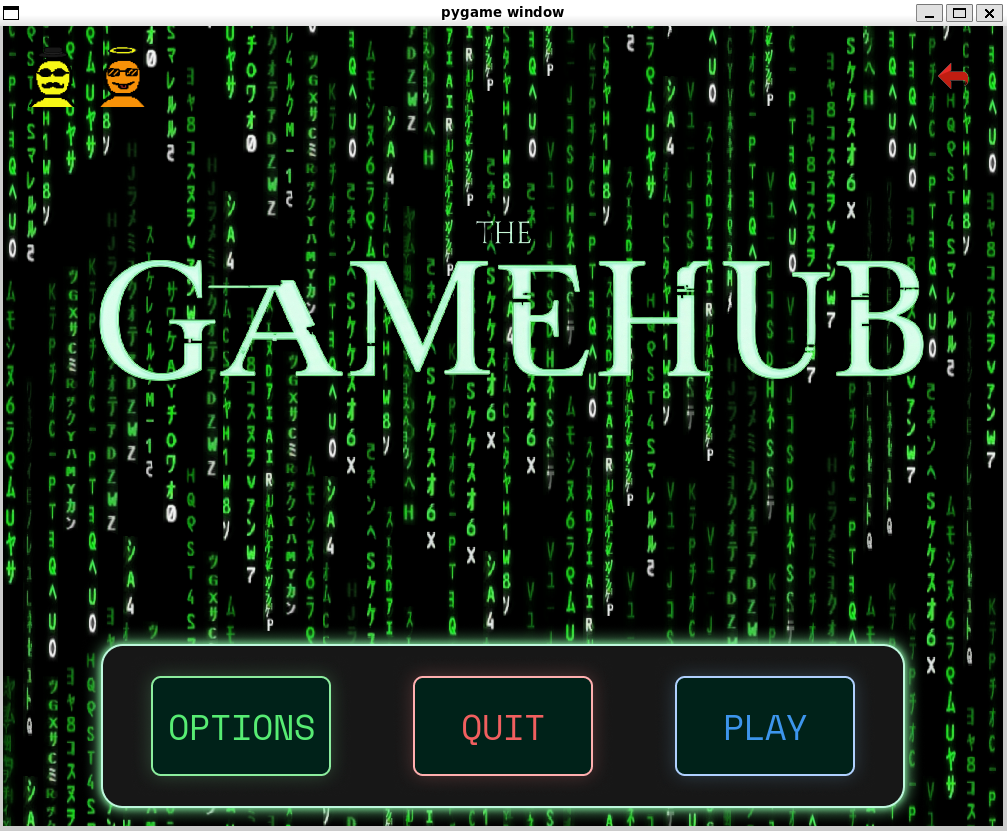
\includegraphics[width=0.75\textwidth]{landingscreen.png}
    \caption{GameHub landing screen}
    \label{fig:landingscreen}
\end{figure}
As seen in Fig. 1, there are three buttons on this screen: Options, Quit and Play. There is also a back button in the top right corner. Pressing Quit or the back button quits the program and halts the running of the python file. Pressing Options or Play opens other sub-menus detailed below.

Upon pressing Options, you are presented with the options menu which has 3 choices - Sound, Avatar and Analytics, and there is also a Back button. Pressing any of these(other than back of course) will open the respective sub-menu of each option. 

Sound has options to change the track currently playing and to change the volume of the song. Avatar has options to change various features of each player's respective avatar. Analytics has options to choose which metric the leaderboard will be sorted by when it is displayed, and a button named Show. If you click show, the command \texttt{bash leaderboard.sh} will be called and the leaderboard for each game will be printed out in the terminal. After this, the matplotlib plot of various game-related statistics will be displayed.

Also, upon pressing Play, you are presented with the play menu which has choices of all the 5 games in the project. Upon pressing any of the game buttons, the corresponding game will open and it can be played between the two players. When the game is completed, a win screen will be displayed with the winner's name and avatar for a few seconds, after which the user will be redirected to the Analytics menu.

\section{Retrospective}
\subsection{Challenges Faced}
\begin{description}
\item[Win Condition]: Coming up with a win condition code which did not require any loops was an interesting challenge which forced us to explore numpy documentation and come up with innovative solutions.
\item[Directory structure and Modularity]: Deciding how to make the code modular and understandable while at the same time ensuring its consistency with the remaining files was not difficult but rather pestering. Missing variables, import issues such as circular imports were some of the issues we had to be wary of.
\end{description}
\subsection{What we would have done differently}
\begin{description}
\item[Animations]: Given more time we would like to add animations to the games to make them more fun and captivating.
\item[Readability]: Make the code more readable and include relevant comments from the beginning. Later on cleaning up the code becomes a difficult task and sometimes the writer also forgets which part of the code did what.
\end{description}

\bibliographystyle{plain}
\bibliography{report}

\end{document}